\documentclass[]{article}
\usepackage{lmodern}
\usepackage{amssymb,amsmath}
\usepackage{ifxetex,ifluatex}
\usepackage{fixltx2e} % provides \textsubscript
\ifnum 0\ifxetex 1\fi\ifluatex 1\fi=0 % if pdftex
  \usepackage[T1]{fontenc}
  \usepackage[utf8]{inputenc}
\else % if luatex or xelatex
  \ifxetex
    \usepackage{mathspec}
  \else
    \usepackage{fontspec}
  \fi
  \defaultfontfeatures{Ligatures=TeX,Scale=MatchLowercase}
\fi
% use upquote if available, for straight quotes in verbatim environments
\IfFileExists{upquote.sty}{\usepackage{upquote}}{}
% use microtype if available
\IfFileExists{microtype.sty}{%
\usepackage{microtype}
\UseMicrotypeSet[protrusion]{basicmath} % disable protrusion for tt fonts
}{}
\usepackage[margin=1in]{geometry}
\usepackage{hyperref}
\PassOptionsToPackage{usenames,dvipsnames}{color} % color is loaded by hyperref
\hypersetup{unicode=true,
            pdftitle={Assessment of the cumulative effects of restoration activities on water quality in Tampa Bay, Florida},
            colorlinks=true,
            linkcolor=Maroon,
            citecolor=Blue,
            urlcolor=blue,
            breaklinks=true}
\urlstyle{same}  % don't use monospace font for urls
\usepackage{graphicx,grffile}
\makeatletter
\def\maxwidth{\ifdim\Gin@nat@width>\linewidth\linewidth\else\Gin@nat@width\fi}
\def\maxheight{\ifdim\Gin@nat@height>\textheight\textheight\else\Gin@nat@height\fi}
\makeatother
% Scale images if necessary, so that they will not overflow the page
% margins by default, and it is still possible to overwrite the defaults
% using explicit options in \includegraphics[width, height, ...]{}
\setkeys{Gin}{width=\maxwidth,height=\maxheight,keepaspectratio}
\IfFileExists{parskip.sty}{%
\usepackage{parskip}
}{% else
\setlength{\parindent}{0pt}
\setlength{\parskip}{6pt plus 2pt minus 1pt}
}
\setlength{\emergencystretch}{3em}  % prevent overfull lines
\providecommand{\tightlist}{%
  \setlength{\itemsep}{0pt}\setlength{\parskip}{0pt}}
\setcounter{secnumdepth}{0}
% Redefines (sub)paragraphs to behave more like sections
\ifx\paragraph\undefined\else
\let\oldparagraph\paragraph
\renewcommand{\paragraph}[1]{\oldparagraph{#1}\mbox{}}
\fi
\ifx\subparagraph\undefined\else
\let\oldsubparagraph\subparagraph
\renewcommand{\subparagraph}[1]{\oldsubparagraph{#1}\mbox{}}
\fi

%%% Use protect on footnotes to avoid problems with footnotes in titles
\let\rmarkdownfootnote\footnote%
\def\footnote{\protect\rmarkdownfootnote}

%%% Change title format to be more compact
\usepackage{titling}

% Create subtitle command for use in maketitle
\newcommand{\subtitle}[1]{
  \posttitle{
    \begin{center}\large#1\end{center}
    }
}

\setlength{\droptitle}{-2em}

  \title{Assessment of the cumulative effects of restoration activities on water
quality in Tampa Bay, Florida}
    \pretitle{\vspace{\droptitle}\centering\huge}
  \posttitle{\par}
    \author{}
    \preauthor{}\postauthor{}
    \date{}
    \predate{}\postdate{}
  
\usepackage{lineno}
\linenumbers
\usepackage{setspace}
\linespread{2}
\usepackage{cleveref}
\usepackage{acronym}
\acrodef{tbep}[TBEP]{Tampa Bay Estuary Program}
\acrodef{chla}[chl-\textit{a}]{chlorophyll \textit{a}}

\begin{document}
\maketitle

\hypertarget{introduction}{%
\section{Introduction}\label{introduction}}

Despite considerable investments over the last four decades in coastal
and estuarine ecosystem restoration (Diefenderfer et al.
\protect\hyperlink{ref-Diefenderfer16}{2016}) these efforts continue to
face many challenges that threaten to impede their success. In the Gulf
of Mexico, chronic and discrete drivers contribute to the difficulty in
restoring and managing coastal ecosystems. For example, the synergistic
effects of widespread chronic coastal urbanization and climate change
impacts may limit habitat management effectiveness in the future
(Enwright et al.~2016). Competing management and policy directives for
flood protection, national commerce and energy development complicate
and prolong efforts to abate coastal hypoxia and other water quality
issues (Rabotyagov et al.~2014; OTHERS). Disputes surrounding fair and
equitable natural resource allocation often result in contentious
implementation plans for the long-term sustainability of coastal
resources (GMFMC 2017). And, discrete tropical storm (Greening and
Janicki (\protect\hyperlink{ref-Greening06}{2006}); MORE RECENT?) and
large-scale pollution events (Beyer et al.~2016) often reset, reverse or
delay progress in restoring coastal ecosystems. These factors create a
complex environment for successful implementation of ecosystem
restoration activities along the Gulf Coast.

Notwithstanding these challenges, the difficulty in rigorously
monitoring and understanding an ecosystem's condition and restoration
trajectory at various spatial and temporal scales further constrain a
recognition of restoration success (Hobbs and Harris 2001). The lack of
long-term environmental monitoring is a primary impediment to
understanding pre- versus post- restoration change (Schiff et al.
\protect\hyperlink{ref-Schiff16}{2016}) -- while also impeding the
recognition of any coastal ecosystem improvements derived from prolonged
management, policy and restoration activities. Where long-term coastal
monitoring programs have been implemented, a broader sense of how
management, policy and restoration activities affect coastal ecosystem
quality can be attained (Borja et al.~2015). Utilizing lessons-learned
from environmental monitoring programs, new frameworks are starting to
emerge to better understand and facilitate the implementation of coastal
restoration ecology from a more informed perspective (Bayraktarov et
al.~2016; Diefenderfer et al.
(\protect\hyperlink{ref-Diefenderfer16}{2016})).

A very large, comprehensive and concerted effort to restore Gulf of
Mexico coastal ecosystems is currently underway (GCERC 2013, 2016).
Primary funding for this effort stems from the legal settlements
resulting from the 2010 Deepwater Horizon oil spill. Funding sources
include: early restoration investments that were made immediately
following the spill, resource damage assessments resulting from the
spill's impact (NRDA, 2016), a record legal settlement of civil and
criminal penalties negotiated between the responsible parties and the US
government with strict US congressional oversight (RESTORE Act), and
matching funds from research, monitoring and restoration practitioners
worldwide. These funds, equating to \textgreater{}\$20B US, present the
Gulf of Mexico community an unprecedented opportunity to revitalize
regional restoration efforts that will span multiple generations (GCERC
2013, 2016). Consequently, the restoration investments being made with
these funds will be highly scrutinized. Better understanding the
environmental outcomes of past investments will help identify how, where
and when future resources should be invested so that the Gulf Coast
community can achieve the highest of restoration success.

Because of the difficulties in demonstrating restoration success, new
tools are needed to help guide and support the implementation of Gulf of
Mexico restoration activities. Here, we present an empirical framework
for evaluating the success of investments in water quality improvement
activities to quantify a potential expectation for changes in water
quality. The framework synthesizes monitoring data across spatiotemporal
scales to demonstrate how the cumulative effects of coastal restoration
activities could improve water quality in an estuary. Data on water
quality and restoration projects in the Tampa Bay area (Florida, USA)
were used to demonstrate application of the analysis framework. Tampa
Bay is the second largest estuary in the Gulf of Mexico and has been
intensively monitored since the mid-1970s. The ecological context of
water quality changes in the Bay is well-described and a comprehensive
history of restoration projects occurring in the watershed is available,
making Tampa Bay an ideal test case for demonstrating and applying a new
evaluation framework. The water quality and restoration data were
evaluated to identify 1) types of restoration activities that produce
the greatest improvements in water quality, and 2) over which time
frames may water quality benefits be teased out of synergistic
restoration acitvities. Changes in chlorophyll-a concentrations, a proxy
for negative eutrophication effects within Tampa Bay (Greening et al.
\protect\hyperlink{ref-Greening2014}{2014}), were used to develop
expectations of water quality changes from restoration activities. The
final product is a decision support tool to evaluate alternative
scenarios of restoration implementation strategies.

\hypertarget{methods}{%
\section{Methods}\label{methods}}

\hypertarget{study-area}{%
\subsection{Study area}\label{study-area}}

Tampa Bay is located on the west-central Gulf coast of Florida and its
watershed is one of the most highly developed regions in Florida
(\cref{fig:map}). More than 60 percent of land within 15 km of the Bay
shoreline is a mix of urban and suburban uses (SWFWMD 2011). The Bay has
been a focal point of economic activity since the 1950s and currently
supports a mix of industrial, domestic, and recreational activities. The
watershed includes one of the largest phosphate production regions in
the country, which is supported by port operations primarily in the
northeast portion of the Bay (Greening and Janicki
\protect\hyperlink{ref-Greening06}{2006}). Water quality data have been
collected since the 1970s when environmental conditions were highly
degraded. Nitrogen loads into the Bay in the mid-1970s have been
estimated as 8.9 x 10\^{}6 kg year-1, most of which came from untreated
wastewater effluent (Greening and Janicki
\protect\hyperlink{ref-Greening06}{2006}). In addition to reduced
aesthetics, environmental conditions associated with hyper-eutrophy were
common and included elevated chlorophyll-a concentrations, increased
occurrence of harmful algal species, low concentrations of bottom water
dissolved oxygen, low water clarity, reduced seagrass coverage, and
declines in fishery yields for both sport and recreational species.
Advanced wastewater treatment operations were implemented at municipal
plants by the early 1980s. These efforts were successful in reducing
nutrients loads to the Bay by 90\%.

\begin{figure}
\centerline{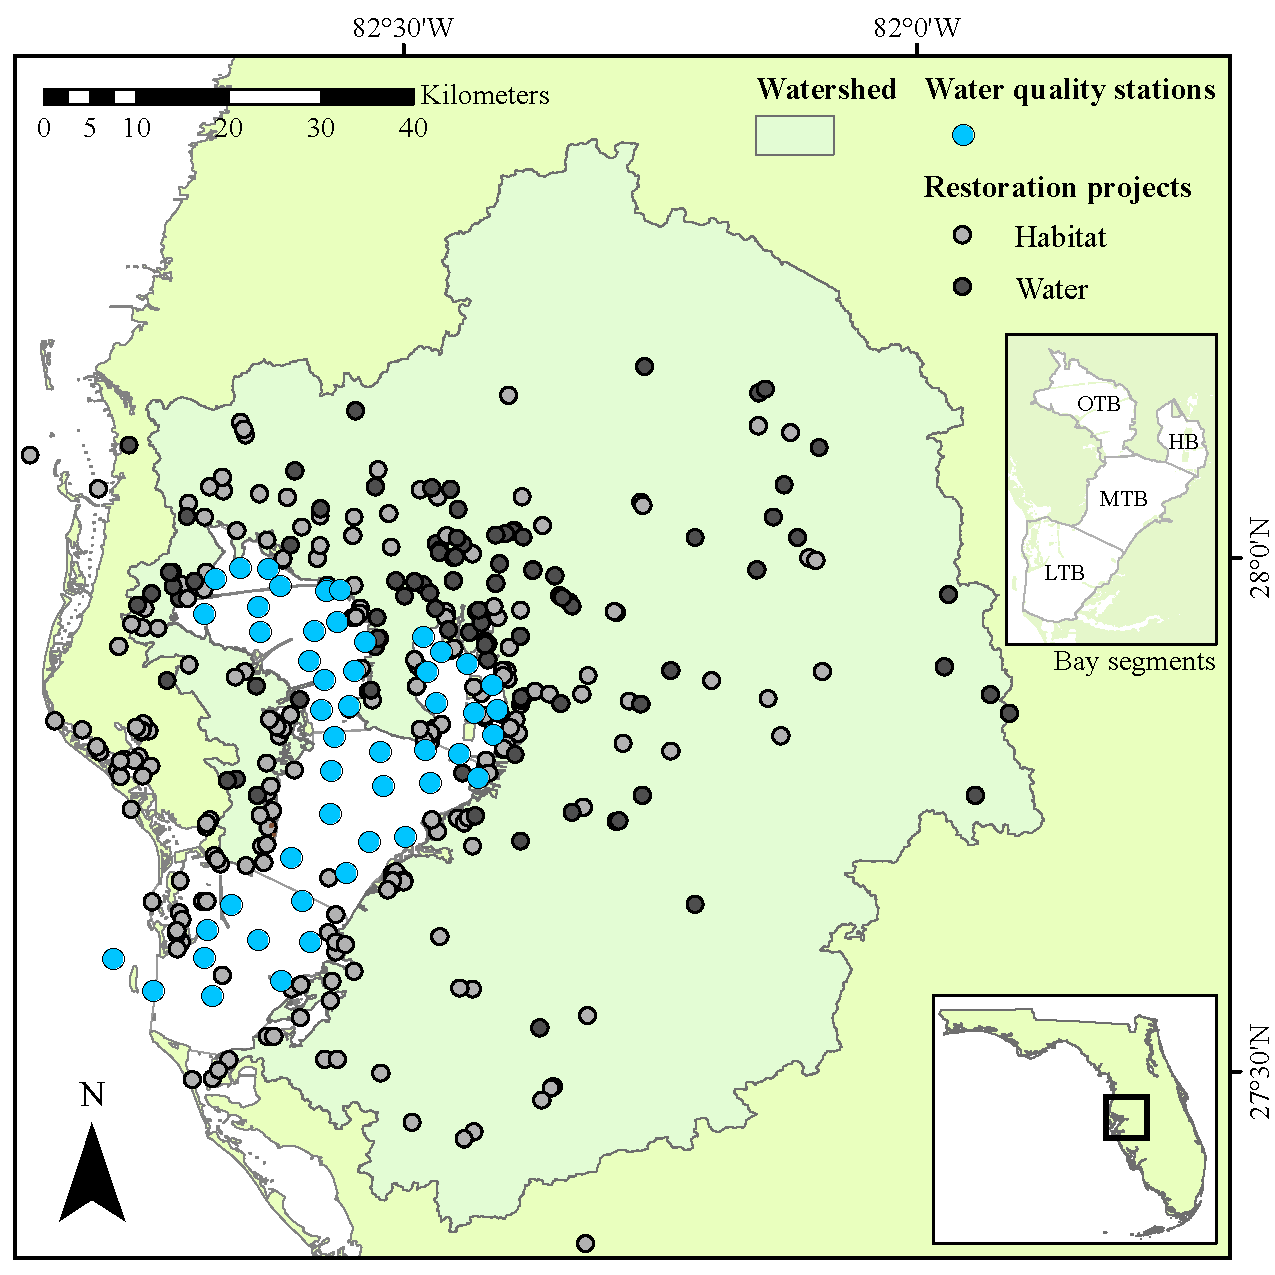
\includegraphics[width = 0.8\textwidth]{figs/tbrest_map.pdf}}
\caption{Water quality stations and restoration projects in the Tampa Bay area.  Water quality stations have been monitored monthly since 1974.  Locations of restoration projects represent 891 records of habitat or water infrastructure projects from 1971 to present.}
\label{fig:map}
\end{figure}

Current water quality in Tampa Bay is dramatically improved from
historical conditions. Most notably, seagrass coverage in 2016 was
reported as 16,857 hectares baywide, surpassing the restoration goal of
coverage in the 1950s (Sherwood et al.
\protect\hyperlink{ref-Sherwood17}{2017}). These changes have occured in
parallel with reductions in nutrient loading (Poe et al.
\protect\hyperlink{ref-Poe05}{2005}; Greening and Janicki
\protect\hyperlink{ref-Greening06}{2006}), chlorophyll concentrations
(Wang, Martin, and Morrison \protect\hyperlink{ref-Wang99}{1999}; Beck
and Hagy III \protect\hyperlink{ref-Beck15}{2015}), and improvements in
water clarity (Morrison et al. \protect\hyperlink{ref-Morrison06}{2006};
Beck, Hagy III, and Le \protect\hyperlink{ref-Beck17c}{2017}). Most of
these positive changes have resulted from management efforts to reduce
point source controls on nutrient pollution in the highly developed
areas of Hillsborough Bay (Johansson
\protect\hyperlink{ref-Johansson91}{1991}; Johansson and Lewis III
\protect\hyperlink{ref-Johansson92}{1992}). However, the cumulative and
synergistic effects of over 800 additional management activities have
likely also contributed to improvements in water quality over time.
Several hundred projects from both public and private entities have been
completed since the 1980s. These projects represent numerous voluntary
(e.g., coastal habitat acquisition, restoration, preservation, etc.) and
compliance-driven (e.g., stormwater retrofits, process water treatment
upgrades, site-level permitting, power plant scrubber upgrades, improved
agricultural practices, etc.) activities. Although it is generally
recognized that these projects have contributed to overall Bay
improvements, the cumulative effects relative to watershed-scale
management efforts are not well understood. Understanding the impacts
within relevant spatial boundaries and how these projects have jointly
contributed to water quality changes over time will provide an improved
understanding of the link between overall estuary improvements and
specific restoration activities.

\hypertarget{data-sources}{%
\subsection{Data sources}\label{data-sources}}

In addition to legacy improvements at wastewater treatment plants,
nearly 900 restoration projects have been documented in the Tampa Bay
area since 1971. Several databases were synthesized to provide a
comprehensive history of projects that have occurred in Tampa Bay and
its watershed. The first dataset was obtained from the Tampa Bay Water
Atlas (version 2.3, \url{http://maps.wateratlas.usf.edu/tampabay/}, TBEP
(Tampa Bay Estuary Program) (\protect\hyperlink{ref-TBEP17}{2017}))
maintained as a joint resource by the University of South Florida and
the \ac{tbep}. This database included 253 projects from 1971 to 2007
that were primarily focused on habitat establishment, enhancement, or
protection in the nearshore areas of the Bay or the larger watershed
(e.g., planting of \emph{Spartina alterniflora}, exotic vegetation
control, etc.). Information on more recent projects (2008-2017) acquired
from the US EPA's National Estuary Program Mapper
(\url{https://gispub2.epa.gov/NEPmap/}) added an additional 265
projects. This database was limited to basic information, such as year
of completion, geographic coordinates, general activities, and areal
coverage. The last database was obtained from the \ac{tbep} Action Plan
Database Portal (\url{https://apdb.tbeptech.org/index.php}) to describe
locations of broader infrastructure improvement projects and structural
best management practices. This database included 368 projects from 1992
to 2016 for county, municipal or industrial activities, such as
implementation of best management practices at treatment plants,
creation of stormwater retention or treatment controls, or site-specific
controls of point sources.

Both project data sources were combined to provide a single dataset
describing the location, year of completion, and project classification
of the restoration activity. The project classifications were described
in two nested categories. The first described a high-level restration
classification for each project as habitat or water infrastructure. The
second was a lower-level classification for habitat projects:
enhancement, establishment, and protection; and water infrastructure
projects: non-point source or point source controls. These categories
were used to provide a broad characterization of restoration activites
that were considered relevant for the perceived improvements in water
quality over time. The nested categories were used to develop separate
models describing the likelihood of changes in water quality (described
below). The final combined dataset included 891 projects from 1971 to
2017 (\cref{fig:restyrs}). Projects with incomplete information (i.e.,
missing date) were not included in the final dataset.

\begin{figure}
\centerline{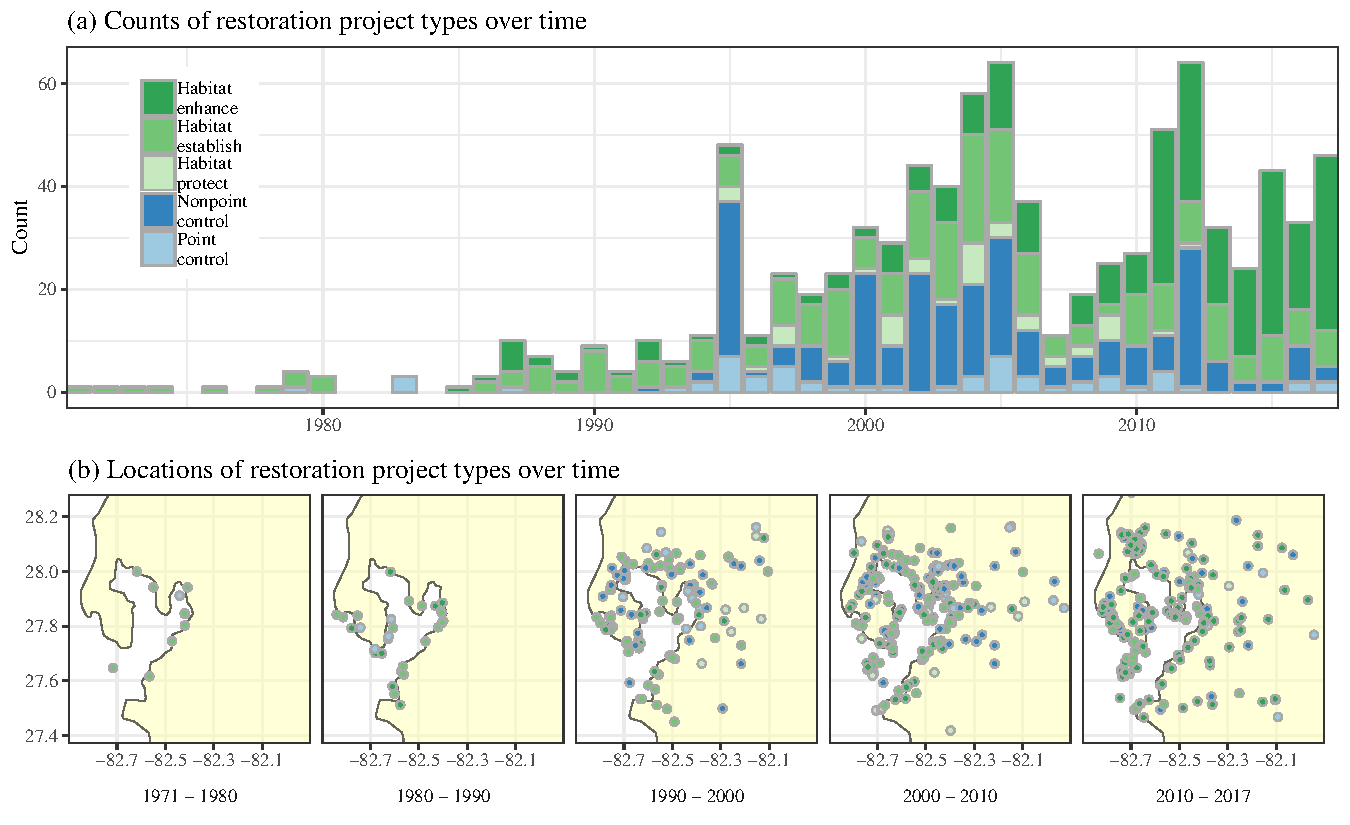
\includegraphics[width = \textwidth]{figs/restyrs.pdf}}
\caption{Counts (top) and locations (bottom) of restoration project types over time in the Tampa Bay watershed.  Restorations were categorized as water infrastructure (nonpoint source controls, point source controls) and habitat (enhancements, establishments, protection) projects.  The compiled restoration database included records of project types and locations from 1971 to 2017.}
\label{fig:restyrs}
\end{figure}

Water quality data in Tampa Bay have been consistently collected since
1974 by the Environmental Protection Commission of Hillsborough County
(TBEP (Tampa Bay Estuary Program) \protect\hyperlink{ref-TBEP17}{2017}).
Data were collected monthly at forty-five stations using a water sample
from mid-depth or a monitoring sonde depending on the parameter.
Monitoring stations are fixed and cover the entire bay from the
uppermost mesohaline sections to the lowermost euhaline portions that
have direct interaction with the Gulf of Mexico. Water samples at each
station are laboratory processed immediately after collection.
Measurements at each site include temperature (C), Secchi disk depth
(m), dissolved oyxgen (mg/L), conductivity (\(\mu\)Ohms/cm), pH,
salinity (psu), turbidity (Nephalometric Turbidy Units), \ac{chla}
(\(\mu\)g/L), total nitrogen (mg/L), and total phosphorus (mg/L). For
the models, all measurements of salinity, total nitrogen, and \ac{chla}
were combined for a total of 515 monthly observations of each parameter
at each station.

\begin{table}[!tbp]
\caption{Summary of total nitrogen and chlorophyll-a observations from monitoring stations in Tampa Bay.  Minimum, median, and maximum observed values for low and high salinity conditions are shown for seasonal and annual aggregations of water quality observations at all monitoring stations (See \cref{fig:map}).  Low or high salinity is based on values below or above 26.5 psu. JFM: January, February, March; AMJ: April, May, June; JAS: July, August, September; OND: October, November, December.\label{tab:statsum}} 
\begin{center}
\begin{tabular}{llllclll}
\hline\hline
\multicolumn{1}{l}{\bfseries Time period}&\multicolumn{3}{c}{\bfseries Total nitrogen}&\multicolumn{1}{c}{\bfseries }&\multicolumn{3}{c}{\bfseries Chlorophyll-a}\tabularnewline
\cline{2-4} \cline{6-8}
\multicolumn{1}{l}{}&\multicolumn{1}{c}{Min}&\multicolumn{1}{c}{Median}&\multicolumn{1}{c}{Max}&\multicolumn{1}{c}{}&\multicolumn{1}{c}{Min}&\multicolumn{1}{c}{Median}&\multicolumn{1}{c}{Max}\tabularnewline
\hline
{\bfseries Low}&&&&&&&\tabularnewline
~~JFM&$0.00$&$0.46$&$2.69$&&$0.12$&$ 5.30$&$114.40$\tabularnewline
~~AMJ&$0.03$&$0.59$&$3.03$&&$0.20$&$ 8.40$&$183.40$\tabularnewline
~~JAS&$0.02$&$0.64$&$3.02$&&$0.50$&$13.80$&$266.60$\tabularnewline
~~OND&$0.03$&$0.57$&$4.14$&&$0.00$&$10.00$&$192.14$\tabularnewline
~~1977-1987&$0.02$&$0.88$&$3.03$&&$0.10$&$13.40$&$266.60$\tabularnewline
~~1987-1997&$0.05$&$0.73$&$4.14$&&$0.00$&$ 8.78$&$192.14$\tabularnewline
~~1997-2007&$0.00$&$0.54$&$2.89$&&$0.12$&$ 7.86$&$261.90$\tabularnewline
~~2007-2017&$0.03$&$0.42$&$2.75$&&$0.50$&$ 7.40$&$220.60$\tabularnewline
\hline
{\bfseries High}&&&&&&&\tabularnewline
~~JFM&$0.03$&$0.43$&$1.65$&&$0.00$&$ 3.20$&$ 55.80$\tabularnewline
~~AMJ&$0.02$&$0.48$&$1.95$&&$0.10$&$ 5.40$&$ 74.90$\tabularnewline
~~JAS&$0.03$&$0.54$&$3.16$&&$0.10$&$ 7.23$&$333.40$\tabularnewline
~~OND&$0.02$&$0.43$&$2.43$&&$0.00$&$ 4.67$&$142.90$\tabularnewline
~~1977-1987&$0.02$&$0.57$&$1.92$&&$0.30$&$ 7.30$&$136.80$\tabularnewline
~~1987-1997&$0.02$&$0.54$&$2.43$&&$0.00$&$ 5.11$&$142.90$\tabularnewline
~~1997-2007&$0.02$&$0.56$&$3.16$&&$0.00$&$ 4.80$&$ 72.30$\tabularnewline
~~2007-2017&$0.03$&$0.33$&$1.80$&&$0.80$&$ 3.70$&$333.40$\tabularnewline
\hline
\end{tabular}\end{center}
\end{table}

\hypertarget{data-synthesis-and-analysis-framework}{%
\subsection{Data synthesis and analysis
framework}\label{data-synthesis-and-analysis-framework}}

Combining the restoration and water quality datasets was a critical part
of developing the analysis framework. Each dataset described events or
sampling activities with unique dates and locations and simple pairing
of restoration projects with water quality data was impractical. To
address this challenge, observations in each dataset were spatially and
temporally matched using an approach designed to maximize the potential
of identifying a unique effect of the restoration projects on changes in
water quality.

\begin{figure}
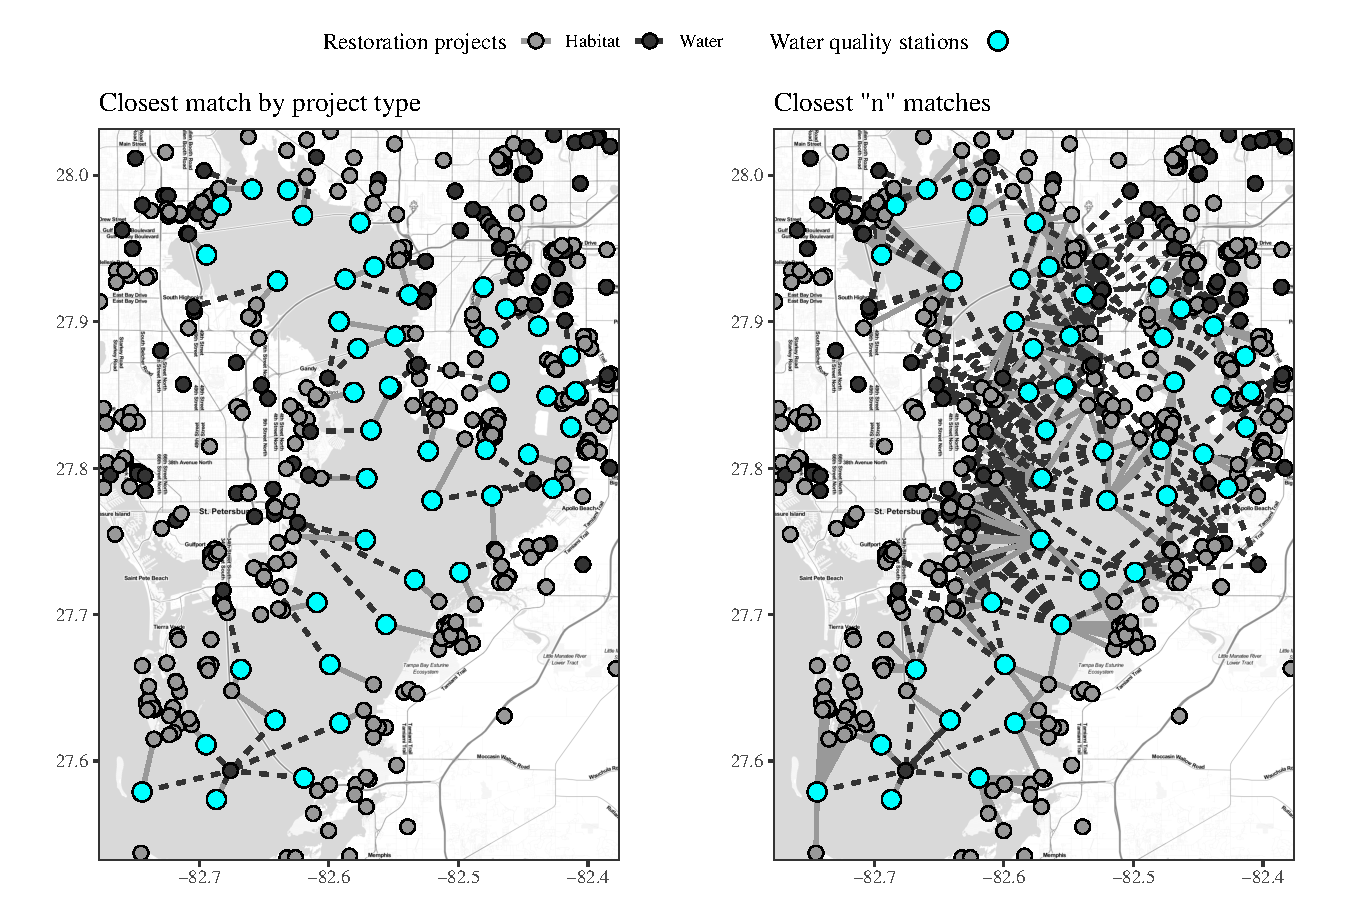
\includegraphics[width=\textwidth]{figs/spmtch} \caption{Spatial matching of water quality stations with restoration projects. Spatial matches of each water quality station with habitat (solid line) and water infrastucture (dashed line) projects are shown as the closest on the left and the "n" closest on the right.  The matchings were repeated for the five restoration project types within the broader habitat and water categories.}\label{fig:spmtch}
\end{figure}

\begin{figure}
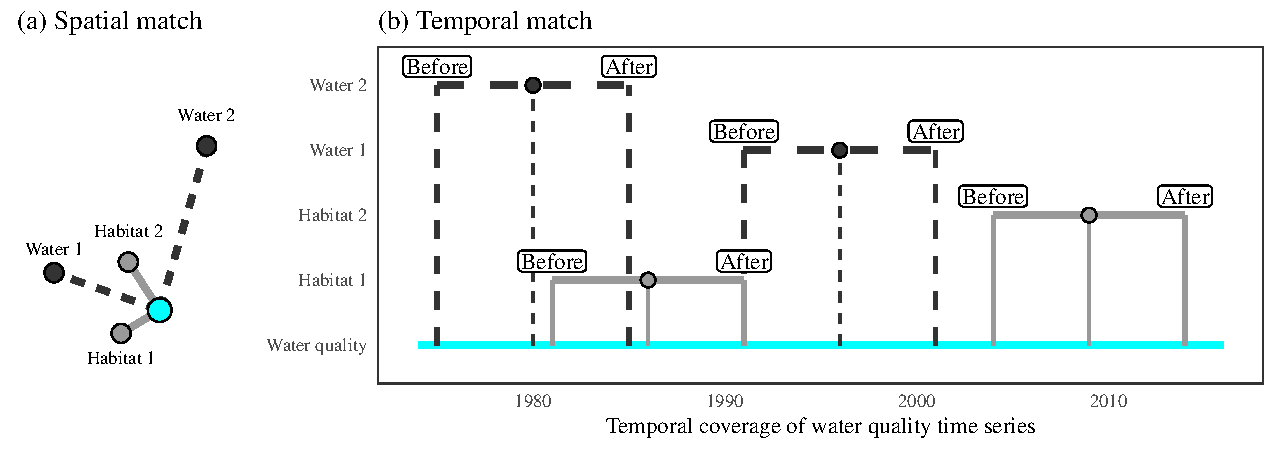
\includegraphics[width=\textwidth]{figs/tmmtch} \caption{Temporal matching of restoration project types with time series data at a water quality station.  The restoration project locations that are spatially matched with a water quality station (a) are used to create a temporal slice of the water quality data within a window of time before and after the completion date of each restoration project (b).  Slices are based on the closest "n" restoration projects by type (n = 2 in this example) to a water quality station.}\label{fig:tmmtch}
\end{figure}

The matching between the two datasets began with a spatial join where
the Euclidean distances between each water quality station and each
restoration project were quantified. The spatial matches were used to
create a ranking of project sites from each water quality station based
on distance. The distances were also grouped by the five restoration
project types (i.e., habitat protection, non-point source control, etc.)
such that the closest \(n\) sites of a given project type could be
identified for any water quality station (\cref{fig:spmtch}). Temporal
matching between water quality stations and restoration projects was
obtained by subsetting the water quality data within a time window
before and after the completion date of each spatially-matched
restoration project (\cref{fig:tmmtch}). For the closest \(n\)
restoration sites for each of five project types, two summarized water
quality estimates were obtained to quantify a before and after effect of
each project. Time windows that overlapped the start and end date of the
water quality time series were discarded. The final two estimates of the
before and after effects of the five types of restoration projects at
each water quality station were based on an average of the \(n\) closest
restoration sites, weighted inversely by distance from the monitoring
station.

Change in water quality relative to each type of restoration project was
estimated as: \begin{equation}
\delta WQ = \frac{\sum_{i = 1}^{n} \hat{wq} \in win + proj_{i, dt}}{n \cdot dist_{i \in n}} - \frac{\sum_{i = 1}^{n} \hat{wq} \in proj_{i, dt} - win}{n \cdot dist_{i \in n}}
\label{eq:wqdif}
\end{equation} where \(\delta WQ\) was the difference between the after
and before averages for each of \(n\) spatially matched restoration
projects. For each \(i\) of \(n\) projects (\(proj\)), the average water
quality (\(\hat{wq}\)) within the window (\(win\)) either before
(\(proj_{i, dt} - win\)) or after (\(win + proj_{i, dt}\)) the
completion date (\(dt\)) for project \(i\) was summed. The summation of
water quality before and after each project was then divided by the
total number of \(n\) matched projects, muliplied by the distance of the
projects from a water quality station (\(dist_{i \in n}\)). This created
a weighted average of the before-after effects of each project that was
inversely related to the distance from a water quality station. A
weighted average by distance was used based on the assumption that
restoration projects farther from a water quality station will have a
weaker signal. The total change in water quality for a project type was
simply the difference in weighted averages. This process was repeated
for every station and a graphical example of \cref{eq:wqdif} is shown in
\cref{fig:statex}

\begin{figure}
\centerline{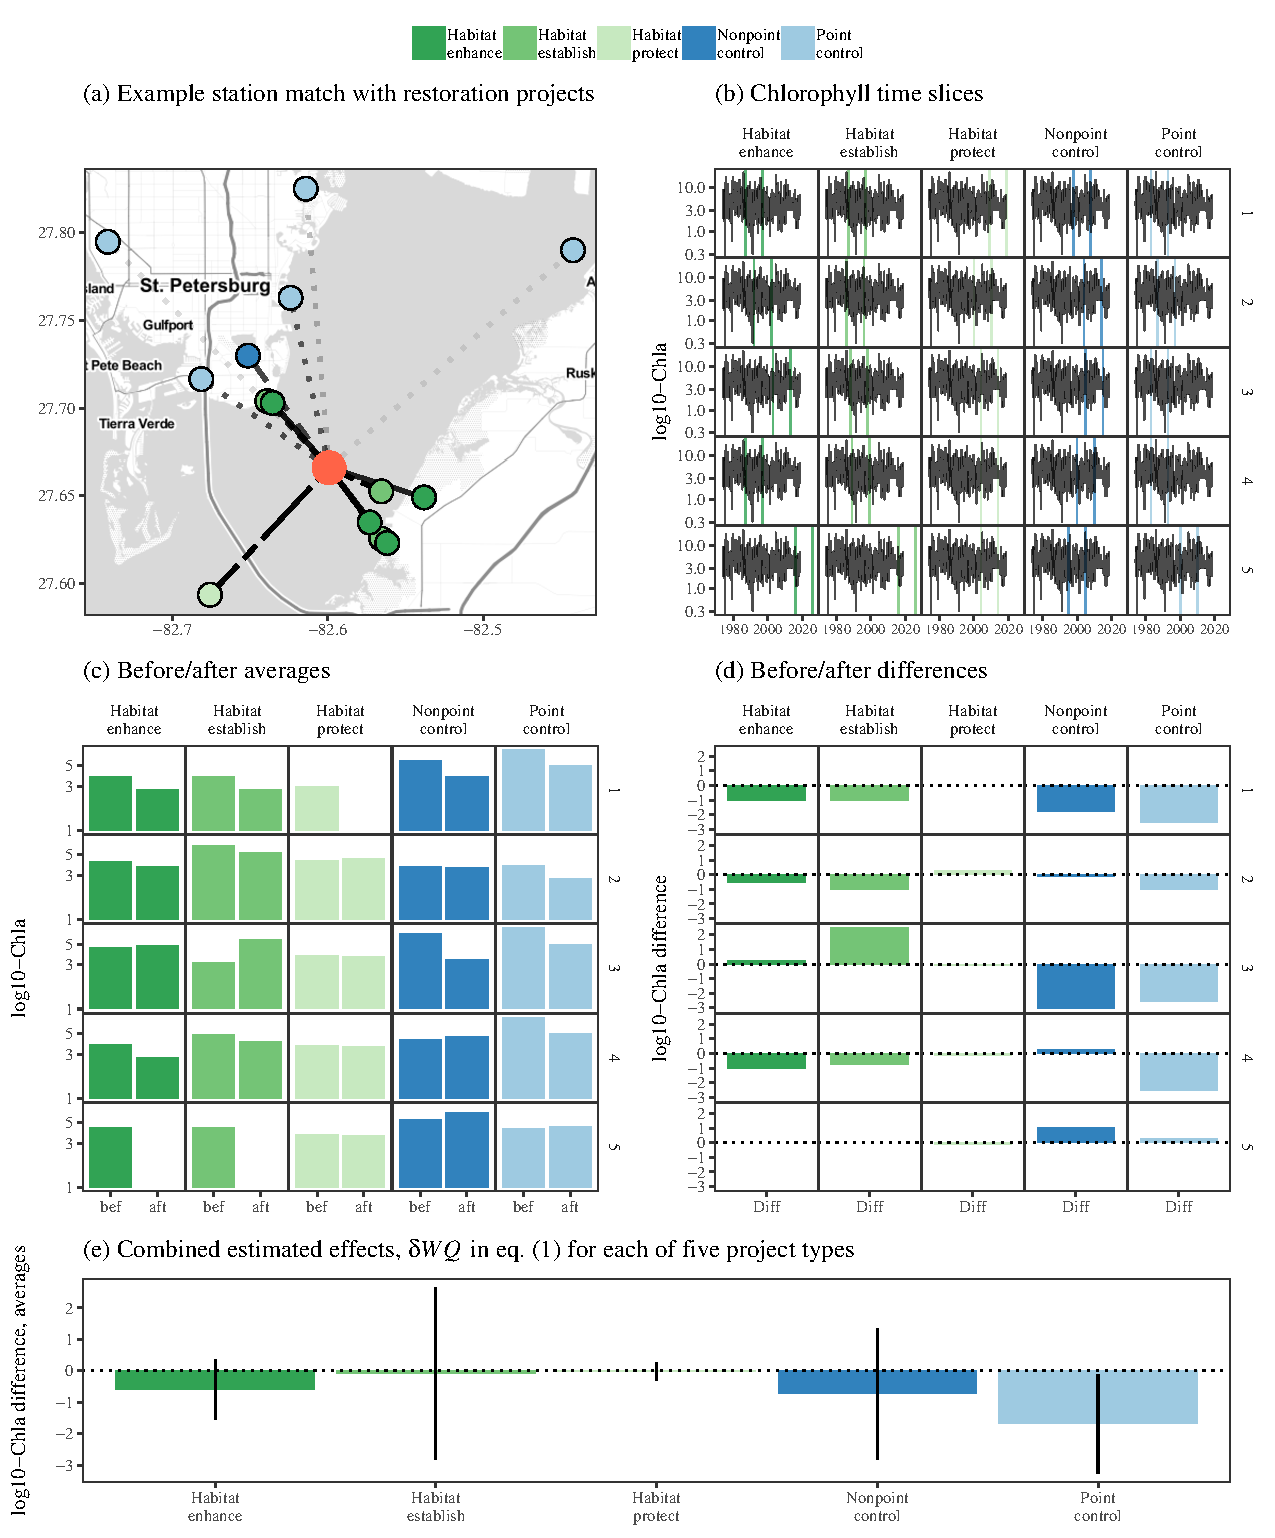
\includegraphics[width = 0.95\textwidth]{figs/statex.pdf}}
\caption{Steps to estimate cumulative effects of water quality changes at a single station relative to a selected number of projects and time windows. Subplot (a) shows station 23 in Middle Tampa Bay matched to the five nearest restoration projects for each of five types.  The time slices of the water quality observations for +/- ten years before and after the completion of each project are shown in (b), ordered from near to far.  The before/after water quality averages for the slices are shown in (c) and the differences between the two are shown in (d).  Finally, the weighted averages for the five closest matches by project type are shown in (e) with 95\% confidence intervals. }
\label{fig:statex}
\end{figure}

The combined water quality and restoration data were used as input for
developing the models. Two parameters in \cref{eq:wqdif} affected the
synthesis of the datasets which directly controlled the ability to
characterize associations of each restoration project type with water
quality changes, 1) \(n\), the number of spatially-matched restoration
projects used to average the cumulative effect of each project type, and
2) \(win\), the time windows before and after a project completion date
that were used to subset each water quality time series. Identifying the
two values that maximized the difference between before and after water
quality measurements was necessary to quantify how many projects induced
a change in water quality, the time within which a change is expected,
and the magnitude of a change differed between project types. Moreover,
two additional factors were also considered that defined the data used
as input in \cref{eq:wqdif}, 1) the total length of the water quality
time series, and 2) the spatial boundaries of the water quality
stations. We evaluated the effects of the length of the time series
(e.g., 1974 to 2017, 1974 to 1994, 1994 to 2017) and the spatial extent
(e.g., whole bay or separate bay segments) to develop a more
comprehensive assessment of the relative associations of each
restoration project type with changes in water quality. This approach
was used given the uneven distribution of restoration projects in space
and time balanced with the known changes in water quality in different
segments of the Bay.

\hypertarget{results}{%
\section{Results}\label{results}}

\hypertarget{initial-data-summaries}{%
\subsection{Initial Data Summaries}\label{initial-data-summaries}}

\hypertarget{chronology-of-restoration-activities}{%
\subsubsection{Chronology of Restoration
Activities}\label{chronology-of-restoration-activities}}

Figure showing restoration types through time.

\hypertarget{observed-water-quality-conditions}{%
\subsubsection{Observed Water Quality
Conditions}\label{observed-water-quality-conditions}}

Table showing seasonal

\hypertarget{assocations-of-restoration-projects-with-water-quality-changes}{%
\subsection{Assocations of restoration projects with water quality
changes}\label{assocations-of-restoration-projects-with-water-quality-changes}}

A figure showing estimated changes across all sites 5, 10 yr windows, 5,
10 projects, maps and boxplots like ind\_eval, repeat for individual
segments

\hypertarget{discussion}{%
\section{Discussion}\label{discussion}}

A long-term record of restoration activities and water quality data in
Tampa Bay provided the foundation to develop a novel decision support
tool for coastal restoration practitioners and managers. This new tool
provides an improved process to understand the expected water quality
improvements that could result from future restoration activities
contingent upon the level of cumulative investments made toward
divergent activities and the required monitoring to understand
downstream water quality benefits at local to watershed-wide scales.
This tool has broad application and extention within the Gulf Coast
restoration and management community. However, several reservations on
its appliction were discovered.

\begin{itemize}
\item
  2004-2017, non-point source and habitat protection appears to have the
  largest effect on chlorophyll-a levels. This effect is not clear until
  after 5 years of monitoring and with the evaluation of multiple
  projects. When fewer restoration activities were taking place in the
  Bay (i.e.~94-04) a greater monitoring time frame was necessary to
  identify the benefits of restoration activities (\textgreater{}5
  years).
\item
  From 1974 - 1994, chlorophyll changes were most distinct in relation
  to water infrastructure projects, particularly for low salinity
  regions in the bay. The effect was more apparent with increasing time
  from the completion of a project and with evaluation of multiple
  projects. Habitat projects did not have a noticeable effect although,
  these were limited to later in the time period.
\item
  It is inherently difficult to determine any downstream water quality
  benefits from enhancement no matter how many sites or years.
  Enhancement is primarily activities such as invasive species removal
  which is not done with the primary goal of improving water quality.
\item
  How can this be used to guide coastal wq management in the Gulf?

  \begin{itemize}
  \tightlist
  \item
    Demonstrate the benefit of Long Term monitoring
  \end{itemize}
\item
  How can this be used to inform or prioritize restoration activities in
  the Gulf?
\item
  What are the limitations of our analysis?
\item
  How can the analysis be applied in other locations?
\end{itemize}

\hypertarget{references}{%
\section*{References}\label{references}}
\addcontentsline{toc}{section}{References}

\hypertarget{refs}{}
\leavevmode\hypertarget{ref-Beck15}{}%
Beck, M. W., and J. D. Hagy III. 2015. ``Adaptation of a Weighted
Regression Approach to Evaluate Water Quality Trends in an Estuary.''
\emph{Environmental Modelling and Assessment} 20 (6):637--55.
\url{https://doi.org/10.1007/s10666-015-9452-8}.

\leavevmode\hypertarget{ref-Beck17c}{}%
Beck, M. W., J. D. Hagy III, and C. Le. 2017. ``Quantifying Seagrass
Light Requirements Using an Algorithm to Spatially Resolve Depth of
Colonization.'' \emph{Estuaries and Coasts}, 1--17.

\leavevmode\hypertarget{ref-Diefenderfer16}{}%
Diefenderfer, Heida L., Gary E. Johnson, Ronald M. Thom, Kate E. Buenau,
Laurie A. Weitkamp, Christa M. Woodley, Amy B. Borde, and Roy K. Kropp.
2016. ``Evidence-Based Evaluation of the Cumulative Effects of Ecosystem
Restoration.'' \emph{Ecosphere} 7 (3):e01242.
\url{http://dx.doi.org/10.1002/ecs2.1242}.

\leavevmode\hypertarget{ref-Greening06}{}%
Greening, H., and A. Janicki. 2006. ``Toward Reversal of Eutrophic
Conditions in a Subtrophical Estuary: Water Quality and Seagrass
Response to Nitrogen Loading Reductions in Tampa Bay, Florida, USA.''
\emph{Environmental Management} 38 (2):163--78.

\leavevmode\hypertarget{ref-Greening2014}{}%
Greening, H S, A Janicki, E T Sherwood, R Pribble, and J O R Johansson.
2014. ``Ecosystem responses to long-term nutrient management in an urban
estuary: Tampa Bay, Florida, USA.'' \emph{Estuarine, Coastal and Shelf
Science} 151 (December):A1--A16.
\url{https://doi.org/10.1016/j.ecss.2014.10.003}.

\leavevmode\hypertarget{ref-Johansson91}{}%
Johansson, J. O. R. 1991. ``Long-Term Trends of Nitrogen Loading, Water
Quality and Biological Indicators in Hillsborough Bay, Florida.'' Edited
by S. F. Treat and P. A. Clark. Tampa, Florida, USA: Tampa Bay Area
Study Group Project at Scholar Commons, 157--76.

\leavevmode\hypertarget{ref-Johansson92}{}%
Johansson, J. O. R., and R. R. Lewis III. 1992. ``Recent Improvements in
Water Quality and Biological Indicators in Hillsborough Bay, a Highly
Impacted Subdivision of Tampa Bay, Florida, USA.'' \emph{Marine Coastal
Eutrophication} Proceedings of an International Conference, Bologna,
Italy, 21-24 March 1990:1199--1215.

\leavevmode\hypertarget{ref-Morrison06}{}%
Morrison, G., E. T. Sherwood, R. Boler, and J. Barron. 2006.
``Variations in Water Clarity and Chlorophyll\emph{a} in Tampa Bay,
Florida, in Response to Annual Rainfall, 1985-2004.'' \emph{Estuaries
and Coasts} 29 (6):926--31.

\leavevmode\hypertarget{ref-Poe05}{}%
Poe, A., K. Hackett, S. Janicki, R. Pribble, and A. Janicki. 2005.
``Estimates of Total Nitrogen, Total Phosphorus, Total Suspended Solids,
and Biochemical Oxygen Demand Loadings to Tampa Bay, Florida:
1999-2003.'' \#02-05. St. Petersburg, Florida, USA: Tampa Bay Estuary
Program.

\leavevmode\hypertarget{ref-Schiff16}{}%
Schiff, K., P.R. Trowbridge, E.T. Sherwood, P. Tango, and R.A. Batiuk.
2016. ``Regional Monitoring Programs in the United States: Synthesis of
Four Case Studies from Pacific, Atlantic, and Gulf Coasts.''
\emph{Regional Studies in Marine Science} 4:A1--A7.
\url{https://doi.org/10.1016/j.rsma.2015.11.007}.

\leavevmode\hypertarget{ref-Sherwood17}{}%
Sherwood, E. T., H. S. Greening, J. O. R. Johansson, K. Kaufman, and G.
Raulerson. 2017. ``Tampa Bay (Florida, USA): Documenting Seagrass
Recovery Since the 1980s and Reviewing the Benefits.''
\emph{Southeastern Geographer} 57 (3):294--319.

\leavevmode\hypertarget{ref-TBEP17}{}%
TBEP (Tampa Bay Estuary Program). 2017. ``Tampa Bay Water Atlas.''

\leavevmode\hypertarget{ref-Wang99}{}%
Wang, P. F., J. Martin, and G. Morrison. 1999. ``Water Quality and
Eutrophication in Tampa Bay, Florida.'' \emph{Estuarine, Coastal and
Shelf Science} 49 (1):1--20.


\end{document}
